\documentclass{article}

\usepackage{graphicx}

\author{Nic Hollingum - 308193415}
\title{Computational Geometry - Assignment 3}

\begin{document}
\maketitle

\section {Voronoi and Trapezoid}

\begin{figure}[htb]
\begin{center}
\leavevmode
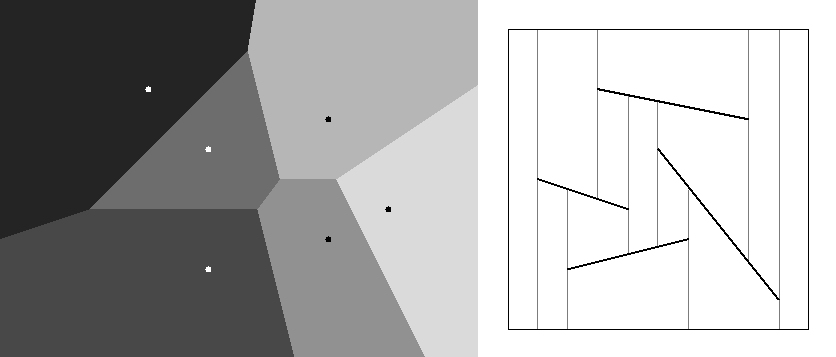
\includegraphics[width=0.9\textwidth]{voronoi.png}
\end{center}
%\caption{Voronoi Segmentation and Trapezoidal Mapping}
\label{fig:vortrap}
\end{figure}

\subsection{a) Voronoi}
A voronoi diagram divides the plane into segments (cells) around the n control points such that any point in $n_i$'s cell is closer to $n_i$ than any other control point.
For large instances, Fortune's algorithm is recommended, which uses a sweep-line technique and runs in $n log n$ time.
However with small instances (such as this) drawing by hand is not so complicated.

A simple way of drawing such a diagram by hand is to mark relative neighbours on the graph and draw a point exactly between them, then extend all points perpendicular to the relative neighbour edge at the same speed.
This particular rendering was done in java where:
\begin{itemize}
	\item for each pixel (x,y).
	\item exhaustively search the points for the closest one.
	\item colour (x,y) with that point's colour.
\end{itemize}

\subsection{b) Trapezoid}
Note, the assignment description sats the 3rd segment lies on $(5,6) \rightarrow (1,9)$, however in the picture it appears (despite being annotated otherwise) to lie on $(5,6) \rightarrow (9,1)$.
We shall go with what the picture says.

This mapping contains 13 trapezoids.
A Trapezoidal Mapping is formed by extending a line up and down at the endpoints of each segment until we reach either the bounding box or another segment.
For simplicity, and indeed in this case, we presume no 2 points share the same x coordinte.

\section {Colinear Points}

\section {Populous Cities}

\section {Trapezoidal Map Size}

\section {Arrangement Bounding}


\end{document}
